\documentclass[10pt,dvipdfmx]{beamer}

\usetheme[progressbar=frametitle]{metropolis}
\usepackage{appendixnumberbeamer}
\usepackage[numbers,sort&compress]{natbib}
\bibliographystyle{plainnat}

\usepackage{amsmath,amssymb,amsthm,ascmac}
\usepackage{booktabs}
\usepackage[scale=2]{ccicons}
\usepackage{bm}
\usepackage{graphicx}
\usepackage{xcolor}
\usepackage{tikz}
\usepackage{geometry}
\usepackage{pgfplots}
\usepackage{xspace}
\newcommand{\themename}{\textbf{\textsc{metropolis}}\xspace}
\usetikzlibrary{patterns}

\title{Supermodularity and Equilibrium in Games with Peer Effects and Endogenous Network Formation}
\subtitle{master's thesis}
\date{\today}
\author{Yuya Furusawa}
\institute{U-Tokyo, GSE}

\begin{document}

\maketitle


\section{Introduction}

\begin{frame}{Network with Peer Effect}
\begin{itemize}
    \item Network structure and local interactions play an important role in individual and aggregate behaviors
    \begin{itemize}
        \item Externalities of the individual behavior in the network is a key factor for the aggeregate bahavior
        \item By considering network structure, we can consider direct effect and indirect effect
    \end{itemize}
    \item Especially, we can see the importance of externalities
    \begin{itemize}
        \item Criminal network, R\&D network, educational network
    \end{itemize}
    \item Many literature argue the importance of "peer effects" theoretically and empirically
\end{itemize}
\end{frame}

\begin{frame}{Endogeneity of the network}
\begin{itemize}
    \item However, in many works, the network is exogenous and fixed
    \item When economic agents are faced with some shocks or policy changes, they respond to them and the network will be changed
\end{itemize}
\end{frame}

\begin{frame}{This paper}
\begin{itemize}
    \item This paper considers the endogenous network formation with peer effects
    \item We consider the model where
    \begin{itemize}
        \item agents first choose the agents who they connect
        \item agents choose the level of effort given the network structure
    \end{itemize}
    \item We provide
    \begin{itemize}
        \item the existence of subgame perfect equilibrium where all agents take pure strategies at each stage
        \item the argument about the equilibrium uniqueness and multiplicity
        \item the discussion about policy implication (key player and key link policy)
    \end{itemize}
\end{itemize}
\end{frame}

\begin{frame}{Related Literature}
\begin{itemize}
    \item Peer effect in networks
    \begin{itemize}
        \item Ballester et.al.(2006), Calv\'{o}-Armengol et.al.(2009), Liu et.al.(2012)
    \end{itemize}
    \item Endogenous network
    \begin{itemize}
        \item Acemoglu and Azar(2019), Oberfield(2018), Farboodi(2014)
    \end{itemize}
    \item Closely related paper(peer effect + endogeneity)
    \begin{itemize}
        \item Kim et.al.(2017), Hiller(2017)
    \end{itemize}
\end{itemize}
\end{frame}


\section{Model}

\begin{frame}{Model : Setup}
\begin{itemize}
    \item the set of agents : $N = \{ 1, \ldots, n \}$ with $n \ge 2$ and $n < \infty$
    \item Agents are initially connected in {\it{potential network}} $\overline{g}$
    \item $\overline{g}$ is represented by adjacency matrix $\bm{\overline{G}} = {(\overline{g}_{ij})}_{ij}$ where
    \[ \overline{g}_{ij} =
        \begin{cases}
            1 \  (\text{if $i$ has a link to $j$ in $\overline{g}$}) \\
            0 \  (\text{otherwise})
        \end{cases} \]
    \item $\bm{\overline{G}}$ need not be symmetric : directed network
    \item Self-loop is not allowed : $\overline{g}_{ii} = 0$ for all $i \in N$
    \item Agent $i$'s neighbors in $\overline{g}$ : $N_i(\overline{g}) = \{ j \in N \mid \overline{g}_{ij} = 1 \}$
\end{itemize}
\end{frame}

\begin{frame}{Model : 1st stage}
\begin{itemize}
    \item First, agents simultaneously choose their neighbors from the agents whom they connect in the potential network
    \item This action is represented by $\psi_i = (\psi_{i1}, \cdots, \psi_{in})$ such that $\psi_{ij} \in \{0, 1\}$ for all $j \in N$, and $\psi_{ij} = 0$ for all $j \notin N_i(\overline{g})$
    \item Denote the agent $i$'s set of actions as $\Psi_i$
    \item The action in the 1st stage is dependent on $\overline{g}$, sometimes we denote $\psi_i(\overline{g})$
    \item When an agent $i$ form link to $j$, he incurs the link-specific costs $c_{ij} \ge 0$
    \begin{itemize}
        \item We denote $\bm{C} = {(c_{ij})}_{ij}$
        \item $\bm{C}$ is not necessarily symmetric
    \end{itemize}
\end{itemize}
\end{frame}

\begin{frame}{Model : 1st stage}
\begin{figure}[h]
\centering
\tikzset{every picture/.style={line width=0.75pt}}
\scalebox{0.7}[0.7]{     
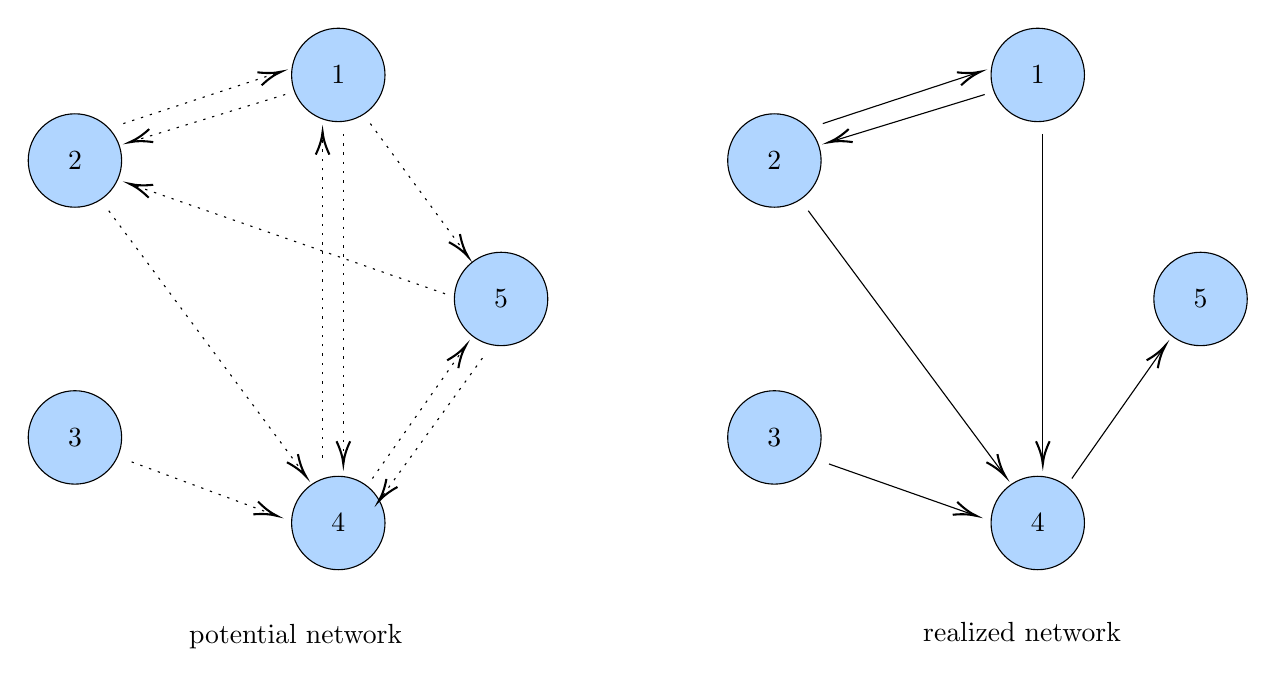
\begin{tikzpicture}[x=0.75pt,y=0.75pt,yscale=-1,xscale=1]
\draw  [fill={rgb, 255:red, 103; green, 174; blue, 255 }  ,fill opacity=0.52 ] (201.07,65.56) .. controls (201.07,53.13) and (211.15,43.06) .. (223.57,43.06) .. controls (236,43.06) and (246.07,53.13) .. (246.07,65.56) .. controls (246.07,77.98) and (236,88.06) .. (223.57,88.06) .. controls (211.15,88.06) and (201.07,77.98) .. (201.07,65.56) -- cycle ;
\draw  [fill={rgb, 255:red, 103; green, 174; blue, 255 }  ,fill opacity=0.52 ] (74.18,106.79) .. controls (74.18,94.36) and (84.25,84.29) .. (96.68,84.29) .. controls (109.1,84.29) and (119.18,94.36) .. (119.18,106.79) .. controls (119.18,119.21) and (109.1,129.29) .. (96.68,129.29) .. controls (84.25,129.29) and (74.18,119.21) .. (74.18,106.79) -- cycle ;
\draw  [fill={rgb, 255:red, 103; green, 174; blue, 255 }  ,fill opacity=0.52 ] (279.5,173.5) .. controls (279.5,161.07) and (289.57,151) .. (302,151) .. controls (314.43,151) and (324.5,161.07) .. (324.5,173.5) .. controls (324.5,185.93) and (314.43,196) .. (302,196) .. controls (289.57,196) and (279.5,185.93) .. (279.5,173.5) -- cycle ;
\draw  [fill={rgb, 255:red, 103; green, 174; blue, 255 }  ,fill opacity=0.52 ] (74.18,240.21) .. controls (74.18,227.79) and (84.25,217.71) .. (96.68,217.71) .. controls (109.1,217.71) and (119.18,227.79) .. (119.18,240.21) .. controls (119.18,252.64) and (109.1,262.71) .. (96.68,262.71) .. controls (84.25,262.71) and (74.18,252.64) .. (74.18,240.21) -- cycle ;
\draw  [fill={rgb, 255:red, 103; green, 174; blue, 255 }  ,fill opacity=0.52 ] (201.07,281.44) .. controls (201.07,269.02) and (211.15,258.94) .. (223.57,258.94) .. controls (236,258.94) and (246.07,269.02) .. (246.07,281.44) .. controls (246.07,293.87) and (236,303.94) .. (223.57,303.94) .. controls (211.15,303.94) and (201.07,293.87) .. (201.07,281.44) -- cycle ;
\draw  [dash pattern={on 0.84pt off 2.51pt}]  (239,89) -- (284.82,151.39) ;
\draw [shift={(286,153)}, rotate = 233.71] [color={rgb, 255:red, 0; green, 0; blue, 0 }  ][line width=0.75]    (10.93,-3.29) .. controls (6.95,-1.4) and (3.31,-0.3) .. (0,0) .. controls (3.31,0.3) and (6.95,1.4) .. (10.93,3.29)   ;
\draw  [dash pattern={on 0.84pt off 2.51pt}]  (198,75) -- (124.91,97.41) ;
\draw [shift={(123,98)}, rotate = 342.95] [color={rgb, 255:red, 0; green, 0; blue, 0 }  ][line width=0.75]    (10.93,-3.29) .. controls (6.95,-1.4) and (3.31,-0.3) .. (0,0) .. controls (3.31,0.3) and (6.95,1.4) .. (10.93,3.29)   ;
\draw  [dash pattern={on 0.84pt off 2.51pt}]  (226,94) -- (226,251) ;
\draw [shift={(226,253)}, rotate = 270] [color={rgb, 255:red, 0; green, 0; blue, 0 }  ][line width=0.75]    (10.93,-3.29) .. controls (6.95,-1.4) and (3.31,-0.3) .. (0,0) .. controls (3.31,0.3) and (6.95,1.4) .. (10.93,3.29)   ;
\draw  [dash pattern={on 0.84pt off 2.51pt}]  (120,89) -- (194.1,64.62) ;
\draw [shift={(196,64)}, rotate = 521.79] [color={rgb, 255:red, 0; green, 0; blue, 0 }  ][line width=0.75]    (10.93,-3.29) .. controls (6.95,-1.4) and (3.31,-0.3) .. (0,0) .. controls (3.31,0.3) and (6.95,1.4) .. (10.93,3.29)   ;
\draw  [dash pattern={on 0.84pt off 2.51pt}]  (113,131) -- (206.81,257.39) ;
\draw [shift={(208,259)}, rotate = 233.42000000000002] [color={rgb, 255:red, 0; green, 0; blue, 0 }  ][line width=0.75]    (10.93,-3.29) .. controls (6.95,-1.4) and (3.31,-0.3) .. (0,0) .. controls (3.31,0.3) and (6.95,1.4) .. (10.93,3.29)   ;
\draw  [dash pattern={on 0.84pt off 2.51pt}]  (124,252) -- (192.13,277.3) ;
\draw [shift={(194,278)}, rotate = 200.38] [color={rgb, 255:red, 0; green, 0; blue, 0 }  ][line width=0.75]    (10.93,-3.29) .. controls (6.95,-1.4) and (3.31,-0.3) .. (0,0) .. controls (3.31,0.3) and (6.95,1.4) .. (10.93,3.29)   ;
\draw  [dash pattern={on 0.84pt off 2.51pt}]  (216,250) -- (216,95) ;
\draw [shift={(216,93)}, rotate = 450] [color={rgb, 255:red, 0; green, 0; blue, 0 }  ][line width=0.75]    (10.93,-3.29) .. controls (6.95,-1.4) and (3.31,-0.3) .. (0,0) .. controls (3.31,0.3) and (6.95,1.4) .. (10.93,3.29)   ;
\draw  [dash pattern={on 0.84pt off 2.51pt}]  (240,260) -- (283.85,197.64) ;
\draw [shift={(285,196)}, rotate = 485.11] [color={rgb, 255:red, 0; green, 0; blue, 0 }  ][line width=0.75]    (10.93,-3.29) .. controls (6.95,-1.4) and (3.31,-0.3) .. (0,0) .. controls (3.31,0.3) and (6.95,1.4) .. (10.93,3.29)   ;
\draw  [dash pattern={on 0.84pt off 2.51pt}]  (293,202) -- (244.17,269.38) ;
\draw [shift={(243,271)}, rotate = 305.93] [color={rgb, 255:red, 0; green, 0; blue, 0 }  ][line width=0.75]    (10.93,-3.29) .. controls (6.95,-1.4) and (3.31,-0.3) .. (0,0) .. controls (3.31,0.3) and (6.95,1.4) .. (10.93,3.29)   ;
\draw  [dash pattern={on 0.84pt off 2.51pt}]  (275,171) -- (124.89,118.66) ;
\draw [shift={(123,118)}, rotate = 379.22] [color={rgb, 255:red, 0; green, 0; blue, 0 }  ][line width=0.75]    (10.93,-3.29) .. controls (6.95,-1.4) and (3.31,-0.3) .. (0,0) .. controls (3.31,0.3) and (6.95,1.4) .. (10.93,3.29)   ;
\draw  [fill={rgb, 255:red, 103; green, 174; blue, 255 }  ,fill opacity=0.52 ] (538.07,65.56) .. controls (538.07,53.13) and (548.15,43.06) .. (560.57,43.06) .. controls (573,43.06) and (583.07,53.13) .. (583.07,65.56) .. controls (583.07,77.98) and (573,88.06) .. (560.57,88.06) .. controls (548.15,88.06) and (538.07,77.98) .. (538.07,65.56) -- cycle ;
\draw  [fill={rgb, 255:red, 103; green, 174; blue, 255 }  ,fill opacity=0.52 ] (411.18,106.79) .. controls (411.18,94.36) and (421.25,84.29) .. (433.68,84.29) .. controls (446.1,84.29) and (456.18,94.36) .. (456.18,106.79) .. controls (456.18,119.21) and (446.1,129.29) .. (433.68,129.29) .. controls (421.25,129.29) and (411.18,119.21) .. (411.18,106.79) -- cycle ;
\draw  [fill={rgb, 255:red, 103; green, 174; blue, 255 }  ,fill opacity=0.52 ] (616.5,173.5) .. controls (616.5,161.07) and (626.57,151) .. (639,151) .. controls (651.43,151) and (661.5,161.07) .. (661.5,173.5) .. controls (661.5,185.93) and (651.43,196) .. (639,196) .. controls (626.57,196) and (616.5,185.93) .. (616.5,173.5) -- cycle ;
\draw  [fill={rgb, 255:red, 103; green, 174; blue, 255 }  ,fill opacity=0.52 ] (411.18,240.21) .. controls (411.18,227.79) and (421.25,217.71) .. (433.68,217.71) .. controls (446.1,217.71) and (456.18,227.79) .. (456.18,240.21) .. controls (456.18,252.64) and (446.1,262.71) .. (433.68,262.71) .. controls (421.25,262.71) and (411.18,252.64) .. (411.18,240.21) -- cycle ;
\draw  [fill={rgb, 255:red, 103; green, 174; blue, 255 }  ,fill opacity=0.52 ] (538.07,281.44) .. controls (538.07,269.02) and (548.15,258.94) .. (560.57,258.94) .. controls (573,258.94) and (583.07,269.02) .. (583.07,281.44) .. controls (583.07,293.87) and (573,303.94) .. (560.57,303.94) .. controls (548.15,303.94) and (538.07,293.87) .. (538.07,281.44) -- cycle ;
\draw    (535,75) -- (461.91,97.41) ;
\draw [shift={(460,98)}, rotate = 342.95] [color={rgb, 255:red, 0; green, 0; blue, 0 }  ][line width=0.75]    (10.93,-3.29) .. controls (6.95,-1.4) and (3.31,-0.3) .. (0,0) .. controls (3.31,0.3) and (6.95,1.4) .. (10.93,3.29)   ;
\draw    (563,94) -- (563,251) ;
\draw [shift={(563,253)}, rotate = 270] [color={rgb, 255:red, 0; green, 0; blue, 0 }  ][line width=0.75]    (10.93,-3.29) .. controls (6.95,-1.4) and (3.31,-0.3) .. (0,0) .. controls (3.31,0.3) and (6.95,1.4) .. (10.93,3.29)   ;
\draw    (457,89) -- (531.1,64.62) ;
\draw [shift={(533,64)}, rotate = 521.79] [color={rgb, 255:red, 0; green, 0; blue, 0 }  ][line width=0.75]    (10.93,-3.29) .. controls (6.95,-1.4) and (3.31,-0.3) .. (0,0) .. controls (3.31,0.3) and (6.95,1.4) .. (10.93,3.29)   ;
\draw    (450,131) -- (543.81,257.39) ;
\draw [shift={(545,259)}, rotate = 233.42000000000002] [color={rgb, 255:red, 0; green, 0; blue, 0 }  ][line width=0.75]    (10.93,-3.29) .. controls (6.95,-1.4) and (3.31,-0.3) .. (0,0) .. controls (3.31,0.3) and (6.95,1.4) .. (10.93,3.29)   ;
\draw    (460,253) -- (529.11,277.34) ;
\draw [shift={(531,278)}, rotate = 199.4] [color={rgb, 255:red, 0; green, 0; blue, 0 }  ][line width=0.75]    (10.93,-3.29) .. controls (6.95,-1.4) and (3.31,-0.3) .. (0,0) .. controls (3.31,0.3) and (6.95,1.4) .. (10.93,3.29)   ;
\draw    (577,260) -- (620.85,197.64) ;
\draw [shift={(622,196)}, rotate = 485.11] [color={rgb, 255:red, 0; green, 0; blue, 0 }  ][line width=0.75]    (10.93,-3.29) .. controls (6.95,-1.4) and (3.31,-0.3) .. (0,0) .. controls (3.31,0.3) and (6.95,1.4) .. (10.93,3.29)   ;
\draw (223.57,65.56) node   {$1$};
\draw (96.68,106.79) node   {$2$};
\draw (96.68,240.21) node   {$3$};
\draw (223.57,281.44) node   {$4$};
\draw (302,173.5) node   {$5$};
\draw (560.57,65.56) node   {$1$};
\draw (433.68,106.79) node   {$2$};
\draw (433.68,240.21) node   {$3$};
\draw (560.57,281.44) node   {$4$};
\draw (639,173.5) node   {$5$};
\draw (203,336) node  [align=left] {potential network};
\draw (553,334) node  [align=left] {realized network};
\end{tikzpicture}}
\caption{Difference between potential network and realized network}
\end{figure}
\end{frame}

\begin{frame}{Model : Realized network}
\begin{itemize}
    \item At the end of the 1st stage, we can see {\it{realized network}} denoted as $g$
    \item $g$ is represented by the adjacency matrix $\bm{G}$
    \[ g_{ij}(\psi_{ij}(\overline{g})) = 
        \begin{cases}
            1 \  (\text{if} \  \psi_{ij}(\overline{g}) = 1 ) \\
            0 \  (\text{otherwise})
        \end{cases} \]
    \item $g$ depends on $\bm{\psi}(\overline{g}) = (\psi_1(\overline{g}), \cdots, \psi_n(\overline{g}))$, so we can denote $g(\bm{\psi}(\overline{g}))$
    \item To avoid redundant expressions, we denote $g(\bm{\psi})$
\end{itemize}
\end{frame}

\begin{frame}{Model : 2nd stage}
\begin{itemize}
    \item Given the realized network, each agent $i \in N$ simultaneously exerts an effort $x_i \ge 0$
    \item Denote $\bm{x} = (x_1, \cdots, x_n)$
    \item Payoff function is
        \[ u_i(\bm{x}, \bm{\psi}, \bm{C}, \phi) = v_i(\bm{x}, g(\bm{\psi}), \phi) - \sum_{j=1}^n g_{ij}(\bm{\psi}) c_{ij} \]
        where
        \[ v_i(\bm{x}, g(\bm{\psi}), \phi) = \alpha_i x_i - \frac{1}{2} x_i^2 + \phi \sum_{j=1}^n g_{ij}(\bm{\psi}) x_i x_j \]
    \item $\phi > 0$ and cross term represent the peer effect
    \item $\alpha_i > 0$ and denote $\bm{\alpha} = (\alpha_1, \cdots, \alpha_n)$
\end{itemize}
\end{frame}

\begin{frame}{Interpretation : Examples}
\begin{itemize}
    \item agent : web sites, municaiparities in Mexico and U.S.
    \item link : ad on other sites, drug traffick
    \item link formation cost : ad fee, prob of capture during trafficking
    \item effort : investments on web contents, drug demand
\end{itemize}
\end{frame}


\section{Equilibrium}

\begin{frame}{Equilibrium}
\begin{itemize}
    \item {\bf{Definition}} : Given $\overline{g}$ and $\bm{C}$, a network $g^*$ is an {\it{equilibrium network}} if $g^* = g(\bm{\psi}^*)$ where $\bm{\psi}^*$ is an action profile in a pure strategy subgame perfect equilibrium.
    \item We focus on a pure strategy equilibrium to consider non-stochastic networks
\end{itemize}
\end{frame}

\begin{frame}{2nd stage equilibrium}
\begin{itemize}
    \item {\bf{Assumption}} : $\phi \rho(\bm{\overline{G}}) < 1$ where $\rho(\cdot)$ is spectral radius
    \item {\bf{Proposition}} : Under Assumption, for any realized network $g$, the subgame has a unique Nash equilibrium $\bm{x}^*$, which is interior and given by
    \[ \bm{x}^*(g, \phi, \bm{\alpha}) = {(\bm{I} - \phi \bm{G})}^{-1} \bm{\alpha} \]
    \item This is based on Ballester, Calv\'{o}-Armengol, and Zenou(2006)
    \item We have
    \[ v_i(\bm{x}^*(g), g, \phi) = \frac{1}{2} {x_i^*(g)}^2 \]
\end{itemize}
\end{frame}

\begin{frame}[label=theorem]{Supermodularity of the reduced game}
\begin{itemize}
    \item By backward induction, given 2nd stage Nash equilibrium, consider the 1st stage game as a normal form game $\Gamma = \langle N, \bm{\Psi}, {(u_i)}_{i \in N} \rangle$
    \item {\bf{Theorem}} : For any $\overline{g}$ and $\bm{C}$, $\Gamma$ is a supermodular game, that is,
        \begin{itemize}
            \item $\bm{\Psi}$ is a sublattice of $\prod_{i=1}^n \mathbb{R}^n$, 
            \item $u_i(\psi_i, \psi_{-i})$ is supermodular in $\psi_i$ on $\Psi_i$ for each $\psi_{-i}$ on $\Psi_{-i}$ for each $i$, and
            \item $u_i(\psi_i, \psi_{-i})$ has increasing differences in $(\psi_i, \psi_{-i})$ on $\Psi_i \times \Psi_{-i}$.
        \end{itemize}
        \hyperlink{proof}{[Proof]}
    \item {\bf{Corollary}} : Equilibrium network always exists
\end{itemize}
\end{frame}

\begin{frame}{Intuition}
\begin{itemize}
    \item {\bf{Strategic complementarity in 2nd stage}} : Given the realized network, if the neighbors exert more efforts, the agent has an incentive to exert more effort by peer effects.
    \item {\bf{Strategic complementarity in 1st stage}} : When agent $i$ forms more links, he exerts more effort by the strategic complementarity in 2nd stage. Agent $i$'s increased effort makes agents who have a link to him exert more efforts, so all agents' level of effort weakly increases. Increasing level of efforts makes the agents to connect more agents.
\end{itemize}
\end{frame}

\begin{frame}{Uniqueness/Multiplicity of the equilibrium}
\begin{itemize}
    \item Equilibrium network is sometimes not unique
    \item {\bf{Example}} : Consider $n = 2$, $\bm{\alpha} = (1, 1)$, and $\bm{\overline{G}} = \left[
    \begin{array}{cc}
        0 & 1 \\
        1 & 0
    \end{array} \right]$.

        Then $\left[
    \begin{array}{cc}
        0 & 1 \\
        1 & 0
    \end{array} \right]$ and $\left[
    \begin{array}{cc}
        0 & 0 \\
        0 & 0
    \end{array} \right]$ can be both equilibrium network for some $c_{12}$ and $c_{21}$.
    \item Payoff matrix is:
        \begin{table}[htb]
          \begin{center}
            \begin{tabular}{|l|l|c|} \hline
              \            & $g_{21} = 1$         & $g_{21} = 0$ \\ \hline
              $g_{12} = 1$ & $\left( \frac{1}{2}{\left( \frac{1}{1 - \phi} \right)}^2 - c_{12}, \frac{1}{2}{\left( \frac{1}{1 - \phi} \right)}^2 - c_{21} \right)$ & $\left( \frac{1}{2} {(1 + \phi)}^2 - c_{12}, \frac{1}{2} \right)$ \\ \hline
              $g_{12} = 0$ & $\left( \frac{1}{2}, \frac{1}{2} {(1 + \phi)}^2 - c_{21} \right)$ & $\left( \frac{1}{2}, \frac{1}{2} \right)$ \\ \hline
            \end{tabular}
          \end{center}
        \end{table}
\end{itemize}
\end{frame}

\begin{frame}{Uniqueness/Multiplicity of the equilibrium}
\begin{figure}[h]
\centering
\tikzset{every picture/.style={line width=0.75pt}}  
\scalebox{0.6}[0.6]{     
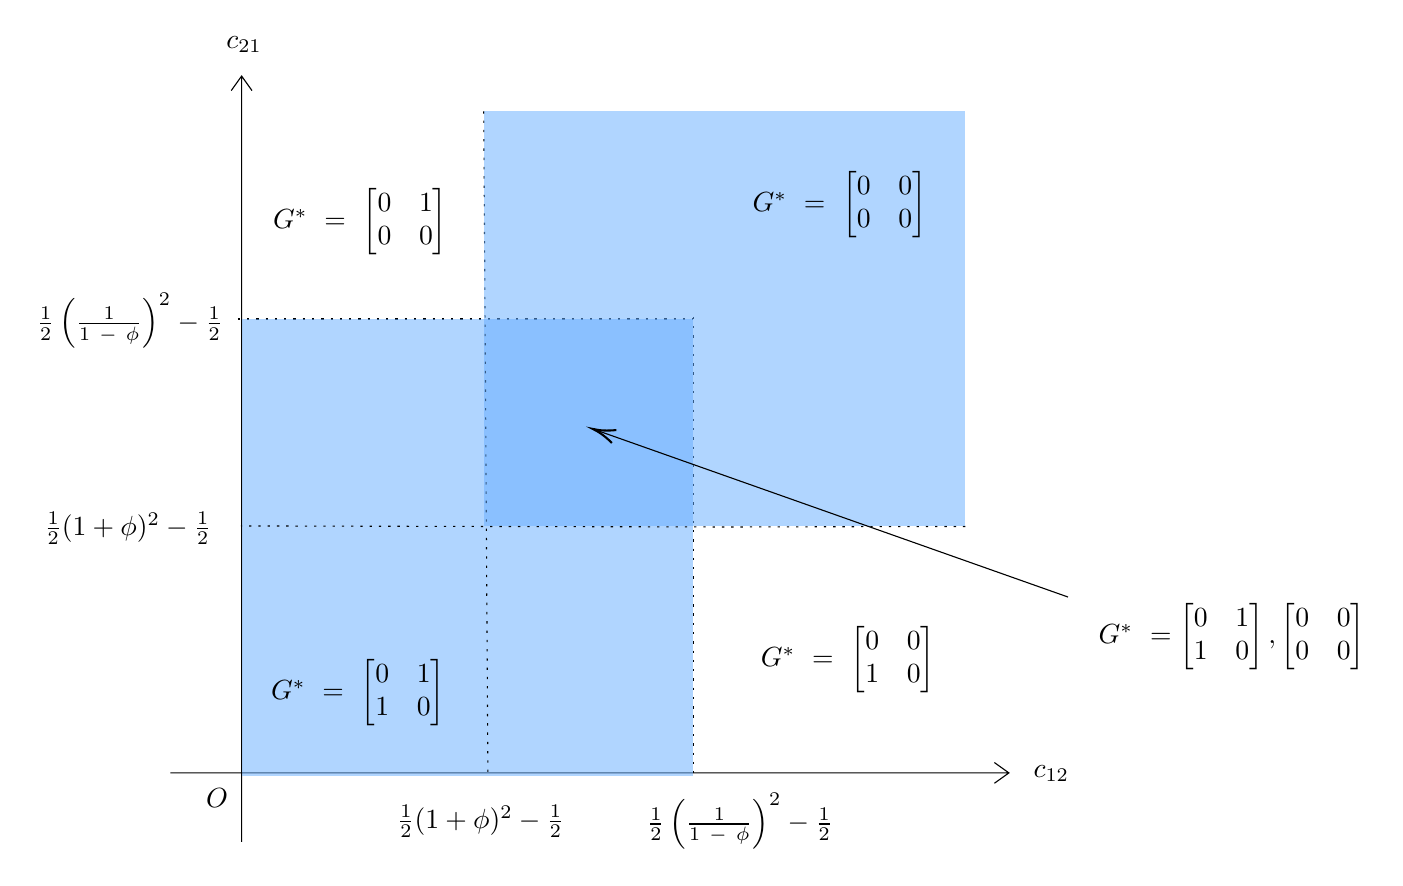
\begin{tikzpicture}[x=0.75pt,y=0.75pt,yscale=-1,xscale=1]
\draw  (115.49,390.74) -- (519.5,390.74)(149.83,55) -- (149.83,423.95) (512.5,385.74) -- (519.5,390.74) -- (512.5,395.74) (144.83,62) -- (149.83,55) -- (154.83,62)  ;
\draw [line width=0.75]  [dash pattern={on 0.84pt off 2.51pt}]  (148,172) -- (367.5,172) ;
\draw  [dash pattern={on 0.84pt off 2.51pt}]  (367.5,171) -- (367.5,392) ;
\draw  [draw opacity=0][fill={rgb, 255:red, 103; green, 174; blue, 255 }  ,fill opacity=0.52 ] (149.83,172) -- (367.5,172) -- (367.5,392) -- (149.83,392) -- cycle ;
\draw  [dash pattern={on 0.84pt off 2.51pt}]  (266.5,72) -- (268.5,392) ;
\draw  [dash pattern={on 0.84pt off 2.51pt}]  (498.5,272) -- (383.5,272.25) -- (149.5,271.75) ;
\draw  [draw opacity=0][fill={rgb, 255:red, 103; green, 174; blue, 255 }  ,fill opacity=0.52 ] (266.5,72) -- (498.5,72) -- (498.5,272) -- (266.5,272) -- cycle ;
\draw    (548,306) -- (320.89,225.67) ;
\draw [shift={(319,225)}, rotate = 379.48] [color={rgb, 255:red, 0; green, 0; blue, 0 }  ][line width=0.75]    (10.93,-3.29) .. controls (6.95,-1.4) and (3.31,-0.3) .. (0,0) .. controls (3.31,0.3) and (6.95,1.4) .. (10.93,3.29)   ;
\draw (540,391) node   {$c_{12}$};
\draw (151,40) node   {$c_{21}$};
\draw (138,403) node   {$O$};
\draw (96,173) node   {$\frac{1}{2}\left(\frac{1}{1\ -\ \phi }\right)^{2} -\frac{1}{2}$};
\draw (390,414) node   {$\frac{1}{2}\left(\frac{1}{1\ -\ \phi }\right)^{2} -\frac{1}{2}$};
\draw (95,273) node   {$\frac{1}{2}( 1+\phi )^{2} -\frac{1}{2}$};
\draw (265,414) node   {$\frac{1}{2}( 1+\phi )^{2} -\frac{1}{2}$};
\draw (438,117) node   {$G^{*} \ =\ \begin{bmatrix}
0 & 0\\
0 & 0
\end{bmatrix}$};
\draw (206,352) node   {$G^{*} \ =\ \begin{bmatrix}
0 & 1\\
1 & 0
\end{bmatrix}$};
\draw (207,125) node   {$G^{*} \ =\ \begin{bmatrix}
0 & 1\\
0 & 0
\end{bmatrix}$};
\draw (442,336) node   {$G^{*} \ =\ \begin{bmatrix}
0 & 0\\
1 & 0
\end{bmatrix}$};
\draw (627,325) node   {$G^{*} \ =\begin{bmatrix}
0 & 1\\
1 & 0
\end{bmatrix} ,\begin{bmatrix}
0 & 0\\
0 & 0
\end{bmatrix}$};
\end{tikzpicture}}
\caption{Equilibrium network region}
\end{figure}
\end{frame}

\begin{frame}{Greatest equilibrium}
\begin{itemize}
    \item By the supermodularity, the greatest and smallest equilibrium network exists
    \item We focus on the greatest equilibrium network and denote $g^{**}$
    \begin{itemize}
        \item The greatest equilibrium can be obtained by sequential {\it{best response dynamics}} which starts from the potential network
    \end{itemize}
\end{itemize}
\end{frame}

\begin{frame}{Comparative Statics}
\begin{itemize}
    \item {\bf{Proposition}} : Given the potential network $\overline{g}$. Consider the cost $\bm{\hat{C}}$ and $\bm{C}$ with $\bm{\hat{C}} \le \bm{C}$. Then,
        \[ g^{**}(\bm{\psi}^*(\overline{g}, \bm{\hat{C}}, \phi, \bm{\alpha})) \supseteq g^{**}(\bm{\psi}^*(\overline{g}, \bm{C}, \phi, \bm{\alpha})) \]
    \item {\bf{Corollary}} : Given the potential network $g^p$. For $\hat{\phi} \ge \phi$ which satisfy the Assumption,
        \[ g^{**}(\bm{\psi}^*(\overline{g}, \bm{C}, \hat{\phi}, \bm{\alpha})) \supseteq g^{**}(\bm{\psi}^*(\overline{g}, \bm{C}, \phi, \bm{\alpha})) \]
        For $\bm{\hat{\alpha}} \ge \bm{\alpha}$,
        \[ g^{**}(\bm{\psi}^*(\overline{g}, \bm{C}, \phi, \bm{\hat{\alpha}})) \supseteq g^{**}(\bm{\psi}^*(\overline{g}, \bm{C}, \phi, \bm{\alpha})) \]
\end{itemize}
\end{frame}

\begin{frame}{Phase transition}
\begin{itemize}
    \item {\bf{Example}} : Suppose $n=5$, $\bm{\alpha} = (1, 1, 1, 1, 1)$, and $\phi = 1/5$
    \item $\bm{C} = \left[
            \begin{array}{ccccc}
                0 & 3 & 3 & 3 & 3 \\
                3 & 0 & 3 & 3 & 3 \\
                3 & 3 & 0 & 3 & 3 \\
                3 & 3 & 3 & 0 & 3  \\
                3 & 3 & 3 & 3 & 0
            \end{array} \right] \Rightarrow \bm{G}^{**} = \left[
            \begin{array}{ccccc}
                0 & 1 & 1 & 1 & 1 \\
                1 & 0 & 1 & 1 & 1 \\
                1 & 1 & 0 & 1 & 1 \\
                1 & 1 & 1 & 0 & 1 \\
                1 & 1 & 1 & 1 & 0
            \end{array} \right]$
    \item $\bm{\hat{C}} = \left[
            \begin{array}{ccccc}
                0 & 3 + \epsilon & 3 & 3 & 3 \\
                3 & 0 & 3 & 3 & 3 \\
                3 & 3 & 0 & 3 & 3 \\
                3 & 3 & 3 & 0 & 3  \\
                3 & 3 & 3 & 3 & 0
            \end{array} \right] \Rightarrow \bm{\hat{G}}^{**} = \left[
            \begin{array}{ccccc}
                0 & 0 & 0 & 0 & 0 \\
                0 & 0 & 0 & 0 & 0 \\
                0 & 0 & 0 & 0 & 0 \\
                0 & 0 & 0 & 0 & 0 \\
                0 & 0 & 0 & 0 & 0
            \end{array} \right]$
\end{itemize}
\end{frame}

\begin{frame}{Phase transition}
\begin{figure}[h]
\centering
\tikzset{every picture/.style={line width=0.75pt}}
\scalebox{0.7}[0.7]{     
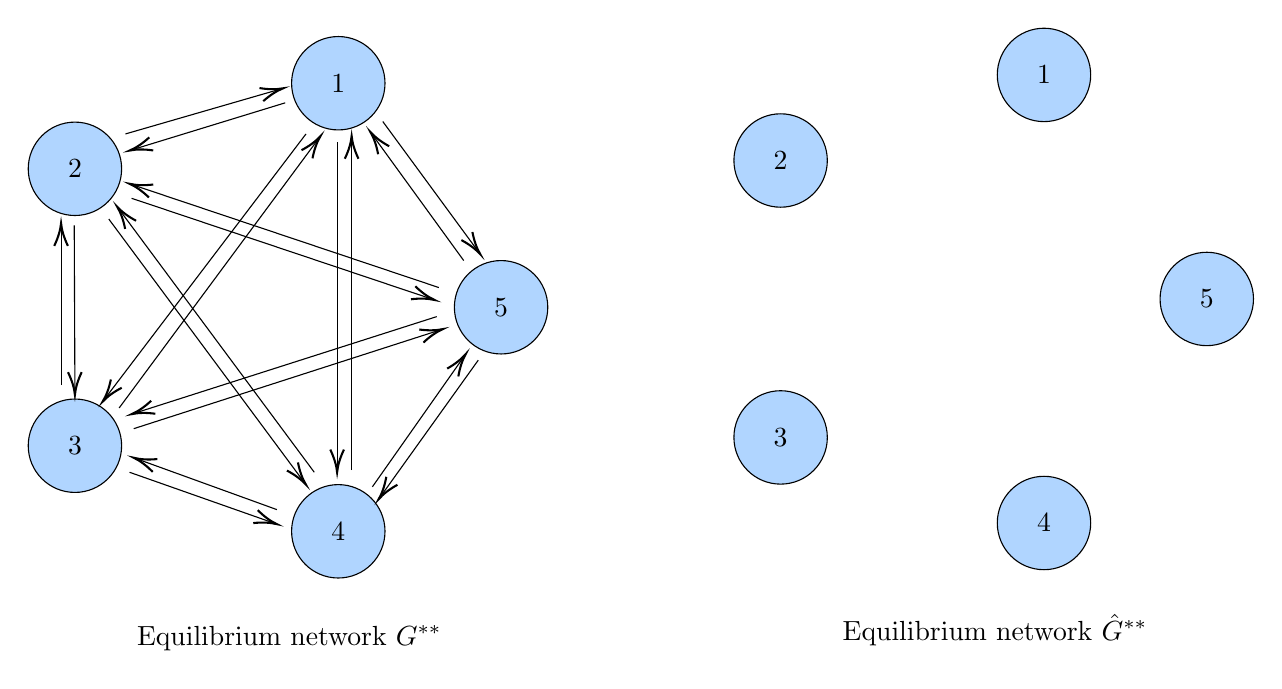
\begin{tikzpicture}[x=0.75pt,y=0.75pt,yscale=-1,xscale=1]
\draw  [fill={rgb, 255:red, 103; green, 174; blue, 255 }  ,fill opacity=0.52 ] (199.07,64.56) .. controls (199.07,52.13) and (209.15,42.06) .. (221.57,42.06) .. controls (234,42.06) and (244.07,52.13) .. (244.07,64.56) .. controls (244.07,76.98) and (234,87.06) .. (221.57,87.06) .. controls (209.15,87.06) and (199.07,76.98) .. (199.07,64.56) -- cycle ;
\draw  [fill={rgb, 255:red, 103; green, 174; blue, 255 }  ,fill opacity=0.52 ] (72.18,105.79) .. controls (72.18,93.36) and (82.25,83.29) .. (94.68,83.29) .. controls (107.1,83.29) and (117.18,93.36) .. (117.18,105.79) .. controls (117.18,118.21) and (107.1,128.29) .. (94.68,128.29) .. controls (82.25,128.29) and (72.18,118.21) .. (72.18,105.79) -- cycle ;
\draw  [fill={rgb, 255:red, 103; green, 174; blue, 255 }  ,fill opacity=0.52 ] (277.5,172.5) .. controls (277.5,160.07) and (287.57,150) .. (300,150) .. controls (312.43,150) and (322.5,160.07) .. (322.5,172.5) .. controls (322.5,184.93) and (312.43,195) .. (300,195) .. controls (287.57,195) and (277.5,184.93) .. (277.5,172.5) -- cycle ;
\draw  [fill={rgb, 255:red, 103; green, 174; blue, 255 }  ,fill opacity=0.52 ] (72.18,239.21) .. controls (72.18,226.79) and (82.25,216.71) .. (94.68,216.71) .. controls (107.1,216.71) and (117.18,226.79) .. (117.18,239.21) .. controls (117.18,251.64) and (107.1,261.71) .. (94.68,261.71) .. controls (82.25,261.71) and (72.18,251.64) .. (72.18,239.21) -- cycle ;
\draw  [fill={rgb, 255:red, 103; green, 174; blue, 255 }  ,fill opacity=0.52 ] (199.07,280.44) .. controls (199.07,268.02) and (209.15,257.94) .. (221.57,257.94) .. controls (234,257.94) and (244.07,268.02) .. (244.07,280.44) .. controls (244.07,292.87) and (234,302.94) .. (221.57,302.94) .. controls (209.15,302.94) and (199.07,292.87) .. (199.07,280.44) -- cycle ;
\draw    (196,74) -- (122.91,96.41) ;
\draw [shift={(121,97)}, rotate = 342.95] [color={rgb, 255:red, 0; green, 0; blue, 0 }  ][line width=0.75]    (10.93,-3.29) .. controls (6.95,-1.4) and (3.31,-0.3) .. (0,0) .. controls (3.31,0.3) and (6.95,1.4) .. (10.93,3.29)   ;
\draw    (221,93) -- (221,250) ;
\draw [shift={(221,252)}, rotate = 270] [color={rgb, 255:red, 0; green, 0; blue, 0 }  ][line width=0.75]    (10.93,-3.29) .. controls (6.95,-1.4) and (3.31,-0.3) .. (0,0) .. controls (3.31,0.3) and (6.95,1.4) .. (10.93,3.29)   ;
\draw    (119,89) -- (193.08,67.56) ;
\draw [shift={(195,67)}, rotate = 523.86] [color={rgb, 255:red, 0; green, 0; blue, 0 }  ][line width=0.75]    (10.93,-3.29) .. controls (6.95,-1.4) and (3.31,-0.3) .. (0,0) .. controls (3.31,0.3) and (6.95,1.4) .. (10.93,3.29)   ;
\draw    (111,130) -- (204.81,256.39) ;
\draw [shift={(206,258)}, rotate = 233.42000000000002] [color={rgb, 255:red, 0; green, 0; blue, 0 }  ][line width=0.75]    (10.93,-3.29) .. controls (6.95,-1.4) and (3.31,-0.3) .. (0,0) .. controls (3.31,0.3) and (6.95,1.4) .. (10.93,3.29)   ;
\draw    (121,252) -- (190.11,276.34) ;
\draw [shift={(192,277)}, rotate = 199.4] [color={rgb, 255:red, 0; green, 0; blue, 0 }  ][line width=0.75]    (10.93,-3.29) .. controls (6.95,-1.4) and (3.31,-0.3) .. (0,0) .. controls (3.31,0.3) and (6.95,1.4) .. (10.93,3.29)   ;
\draw    (238,259) -- (281.85,196.64) ;
\draw [shift={(283,195)}, rotate = 485.11] [color={rgb, 255:red, 0; green, 0; blue, 0 }  ][line width=0.75]    (10.93,-3.29) .. controls (6.95,-1.4) and (3.31,-0.3) .. (0,0) .. controls (3.31,0.3) and (6.95,1.4) .. (10.93,3.29)   ;
\draw    (243,83) -- (288.82,145.39) ;
\draw [shift={(290,147)}, rotate = 233.71] [color={rgb, 255:red, 0; green, 0; blue, 0 }  ][line width=0.75]    (10.93,-3.29) .. controls (6.95,-1.4) and (3.31,-0.3) .. (0,0) .. controls (3.31,0.3) and (6.95,1.4) .. (10.93,3.29)   ;
\draw    (206,89) -- (109.21,216.41) ;
\draw [shift={(108,218)}, rotate = 307.22] [color={rgb, 255:red, 0; green, 0; blue, 0 }  ][line width=0.75]    (10.93,-3.29) .. controls (6.95,-1.4) and (3.31,-0.3) .. (0,0) .. controls (3.31,0.3) and (6.95,1.4) .. (10.93,3.29)   ;
\draw    (94.35,133) -- (94.67,212.71) ;
\draw [shift={(94.68,214.71)}, rotate = 269.77] [color={rgb, 255:red, 0; green, 0; blue, 0 }  ][line width=0.75]    (10.93,-3.29) .. controls (6.95,-1.4) and (3.31,-0.3) .. (0,0) .. controls (3.31,0.3) and (6.95,1.4) .. (10.93,3.29)   ;
\draw    (122,120) -- (266.1,168.36) ;
\draw [shift={(268,169)}, rotate = 198.55] [color={rgb, 255:red, 0; green, 0; blue, 0 }  ][line width=0.75]    (10.93,-3.29) .. controls (6.95,-1.4) and (3.31,-0.3) .. (0,0) .. controls (3.31,0.3) and (6.95,1.4) .. (10.93,3.29)   ;
\draw    (116,221) -- (211.81,91.61) ;
\draw [shift={(213,90)}, rotate = 486.52] [color={rgb, 255:red, 0; green, 0; blue, 0 }  ][line width=0.75]    (10.93,-3.29) .. controls (6.95,-1.4) and (3.31,-0.3) .. (0,0) .. controls (3.31,0.3) and (6.95,1.4) .. (10.93,3.29)   ;
\draw    (88,210) -- (88,134) ;
\draw [shift={(88,132)}, rotate = 450] [color={rgb, 255:red, 0; green, 0; blue, 0 }  ][line width=0.75]    (10.93,-3.29) .. controls (6.95,-1.4) and (3.31,-0.3) .. (0,0) .. controls (3.31,0.3) and (6.95,1.4) .. (10.93,3.29)   ;
\draw    (123,231) -- (270.1,183.61) ;
\draw [shift={(272,183)}, rotate = 522.14] [color={rgb, 255:red, 0; green, 0; blue, 0 }  ][line width=0.75]    (10.93,-3.29) .. controls (6.95,-1.4) and (3.31,-0.3) .. (0,0) .. controls (3.31,0.3) and (6.95,1.4) .. (10.93,3.29)   ;
\draw    (228,251) -- (228,92) ;
\draw [shift={(228,90)}, rotate = 450] [color={rgb, 255:red, 0; green, 0; blue, 0 }  ][line width=0.75]    (10.93,-3.29) .. controls (6.95,-1.4) and (3.31,-0.3) .. (0,0) .. controls (3.31,0.3) and (6.95,1.4) .. (10.93,3.29)   ;
\draw    (116.19,125.61) -- (210,252) ;
\draw [shift={(115,124)}, rotate = 53.42] [color={rgb, 255:red, 0; green, 0; blue, 0 }  ][line width=0.75]    (10.93,-3.29) .. controls (6.95,-1.4) and (3.31,-0.3) .. (0,0) .. controls (3.31,0.3) and (6.95,1.4) .. (10.93,3.29)   ;
\draw    (192,270) -- (124.88,245.68) ;
\draw [shift={(123,245)}, rotate = 379.91999999999996] [color={rgb, 255:red, 0; green, 0; blue, 0 }  ][line width=0.75]    (10.93,-3.29) .. controls (6.95,-1.4) and (3.31,-0.3) .. (0,0) .. controls (3.31,0.3) and (6.95,1.4) .. (10.93,3.29)   ;
\draw    (282,150) -- (238.17,89.62) ;
\draw [shift={(237,88)}, rotate = 414.03] [color={rgb, 255:red, 0; green, 0; blue, 0 }  ][line width=0.75]    (10.93,-3.29) .. controls (6.95,-1.4) and (3.31,-0.3) .. (0,0) .. controls (3.31,0.3) and (6.95,1.4) .. (10.93,3.29)   ;
\draw    (270,163) -- (122.9,113.64) ;
\draw [shift={(121,113)}, rotate = 378.55] [color={rgb, 255:red, 0; green, 0; blue, 0 }  ][line width=0.75]    (10.93,-3.29) .. controls (6.95,-1.4) and (3.31,-0.3) .. (0,0) .. controls (3.31,0.3) and (6.95,1.4) .. (10.93,3.29)   ;
\draw    (269,177) -- (123.9,223.39) ;
\draw [shift={(122,224)}, rotate = 342.27] [color={rgb, 255:red, 0; green, 0; blue, 0 }  ][line width=0.75]    (10.93,-3.29) .. controls (6.95,-1.4) and (3.31,-0.3) .. (0,0) .. controls (3.31,0.3) and (6.95,1.4) .. (10.93,3.29)   ;
\draw    (289,198) -- (242.16,263.37) ;
\draw [shift={(241,265)}, rotate = 305.62] [color={rgb, 255:red, 0; green, 0; blue, 0 }  ][line width=0.75]    (10.93,-3.29) .. controls (6.95,-1.4) and (3.31,-0.3) .. (0,0) .. controls (3.31,0.3) and (6.95,1.4) .. (10.93,3.29)   ;
\draw  [fill={rgb, 255:red, 103; green, 174; blue, 255 }  ,fill opacity=0.52 ] (539.07,60.56) .. controls (539.07,48.13) and (549.15,38.06) .. (561.57,38.06) .. controls (574,38.06) and (584.07,48.13) .. (584.07,60.56) .. controls (584.07,72.98) and (574,83.06) .. (561.57,83.06) .. controls (549.15,83.06) and (539.07,72.98) .. (539.07,60.56) -- cycle ;
\draw  [fill={rgb, 255:red, 103; green, 174; blue, 255 }  ,fill opacity=0.52 ] (412.18,101.79) .. controls (412.18,89.36) and (422.25,79.29) .. (434.68,79.29) .. controls (447.1,79.29) and (457.18,89.36) .. (457.18,101.79) .. controls (457.18,114.21) and (447.1,124.29) .. (434.68,124.29) .. controls (422.25,124.29) and (412.18,114.21) .. (412.18,101.79) -- cycle ;
\draw  [fill={rgb, 255:red, 103; green, 174; blue, 255 }  ,fill opacity=0.52 ] (617.5,168.5) .. controls (617.5,156.07) and (627.57,146) .. (640,146) .. controls (652.43,146) and (662.5,156.07) .. (662.5,168.5) .. controls (662.5,180.93) and (652.43,191) .. (640,191) .. controls (627.57,191) and (617.5,180.93) .. (617.5,168.5) -- cycle ;
\draw  [fill={rgb, 255:red, 103; green, 174; blue, 255 }  ,fill opacity=0.52 ] (412.18,235.21) .. controls (412.18,222.79) and (422.25,212.71) .. (434.68,212.71) .. controls (447.1,212.71) and (457.18,222.79) .. (457.18,235.21) .. controls (457.18,247.64) and (447.1,257.71) .. (434.68,257.71) .. controls (422.25,257.71) and (412.18,247.64) .. (412.18,235.21) -- cycle ;
\draw  [fill={rgb, 255:red, 103; green, 174; blue, 255 }  ,fill opacity=0.52 ] (539.07,276.44) .. controls (539.07,264.02) and (549.15,253.94) .. (561.57,253.94) .. controls (574,253.94) and (584.07,264.02) .. (584.07,276.44) .. controls (584.07,288.87) and (574,298.94) .. (561.57,298.94) .. controls (549.15,298.94) and (539.07,288.87) .. (539.07,276.44) -- cycle ;
\draw (221.57,64.56) node   {$1$};
\draw (94.68,105.79) node   {$2$};
\draw (94.68,239.21) node   {$3$};
\draw (221.57,280.44) node   {$4$};
\draw (300,172.5) node   {$5$};
\draw (198,332) node  [align=left] {Equilibrium network $\displaystyle G^{**}$};
\draw (561.57,60.56) node   {$1$};
\draw (434.68,101.79) node   {$2$};
\draw (434.68,235.21) node   {$3$};
\draw (561.57,276.44) node   {$4$};
\draw (640,168.5) node   {$5$};
\draw (538,328) node  [align=left] {Equilibrium network $\displaystyle \hat{G}^{**}$};
\end{tikzpicture}}
\caption{Equilibrium networks}
\end{figure}
\end{frame}


\section{Policy Implication}

\begin{frame}{Key player}
\begin{itemize}
    \item Key player is the agent who has the largest impact on the aggregate behavior of the network
    \item {\bf{Definition}} : Agent $i$ is a {\it{key player in exogenous network }} if, given network $g$,
        \[ i \in \arg \max_{i \in N} \{ x^*(g) - x^*(g^{-i}) \} \]
        where $x^*(g) = \sum_{i=1}^n x_i^*(g)$ and $g^{-i}$ is the network where agent $i$ is removed from the network $g$
\end{itemize}
\end{frame}

\begin{frame}{Key player in endogenous network}
\begin{itemize}
    \item {\bf{Definition}} : Agent $i$ is a {\it{key player in endogenous network}} if, given potential network $\overline{g}$,
        \[ i \in \arg \max_{i \in N} \{ x^*(g^{**}(\bm{\psi}(\overline{g}, \bm{C}))) - x^*(g^{**}(\bm{\psi}(\overline{g}^{-i}, \bm{C}^{-i}))) \} \]
        where ${\overline{g}}^{-i}$ is the network where agent $i$ is removed from the network $\overline{g}$
    \item However, it is difficult to identify a key player due to the complexity of the mapping from cost structure to realized network
\end{itemize}
\end{frame}

\begin{frame}{Difference bet. endogenous and exogenous key player}
\begin{itemize}
    \item {\bf{Example}} : Suppose $n=5$, $\bm{\alpha} = (1, 1, 1, 1, 1)$ and $\phi = 1/5$
    \item $\bm{C} = \left[
            \begin{array}{ccccc}
                0 & 3.6 & 0.2 & 0.2 & 0.2 \\
                0.3 & 0 & 0.2 & 0.5 & 5.5 \\
                0.2 & 0.2 & 0 & 4.5 & 4.3 \\
                4.1 & 0.2 & 0.4 & 0 & 6.5 \\
                3.2 & 4.1 & 0.3 & 1.0 & 0
            \end{array} \right] \Rightarrow \bm{G}^{**} = \left[
            \begin{array}{ccccc}
                0 & 0 & 1 & 1 & 1 \\
                1 & 0 & 1 & 1 & 0 \\
                1 & 1 & 0 & 0 & 0 \\
                0 & 1 & 1 & 0 & 0 \\
                0 & 0 & 1 & 0 & 0
            \end{array} \right]$
    \item Then,
        \begin{table}[htb]
          \begin{center}
            \begin{tabular}{|l|l|c|} \hline
              agent $1$ & $x_1^* = 1.99541284$ & key player in endogenous network \\ \hline
              agent $2$ & $x_2^* = 2.12155963$ & agent with highest effort \\ \hline
              agent $3$ & $x_3^* = 1.82339450$  & key player in exogenous network \\ \hline
              agent $4$ & $x_4^* = 1.78899083$ & \  \\ \hline
              agent $5$ & $x_5^* = 1.36467890$ & \ \\ \hline
            \end{tabular}
          \end{center}
        \end{table}
\end{itemize}
\end{frame}

\begin{frame}{Diff bet. endogenous and exogenous key player}
\begin{figure}[h]
\raggedleft
\tikzset{every picture/.style={line width=0.75pt}}
\scalebox{0.75}[0.75]{   
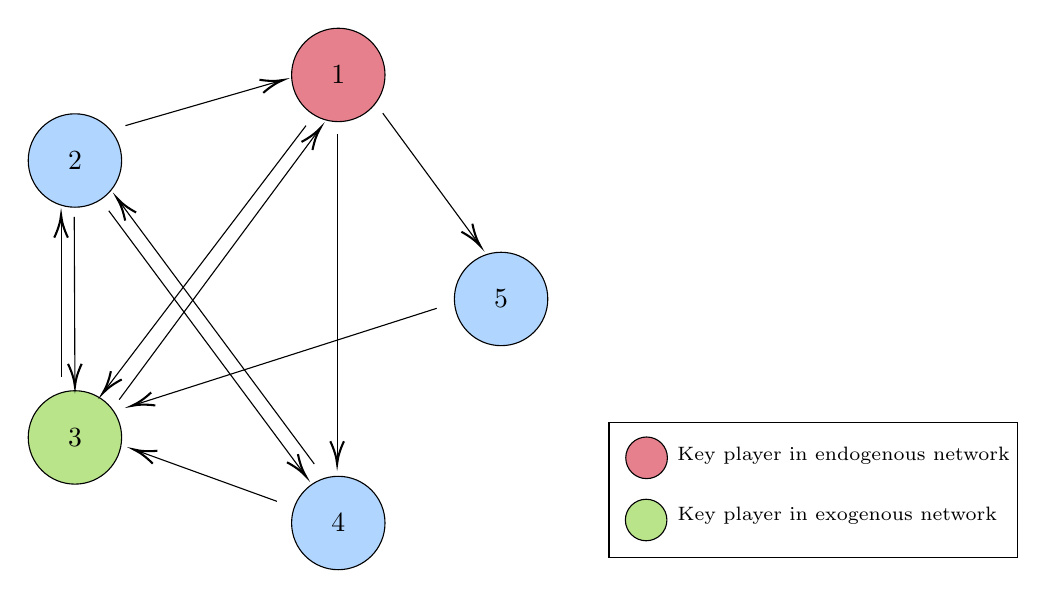
\begin{tikzpicture}[x=0.75pt,y=0.75pt,yscale=-1,xscale=1]
\draw  [fill={rgb, 255:red, 208; green, 2; blue, 27 }  ,fill opacity=0.5 ] (416.07,67.56) .. controls (416.07,55.13) and (426.15,45.06) .. (438.57,45.06) .. controls (451,45.06) and (461.07,55.13) .. (461.07,67.56) .. controls (461.07,79.98) and (451,90.06) .. (438.57,90.06) .. controls (426.15,90.06) and (416.07,79.98) .. (416.07,67.56) -- cycle ;
\draw  [fill={rgb, 255:red, 103; green, 174; blue, 255 }  ,fill opacity=0.52 ] (289.18,108.79) .. controls (289.18,96.36) and (299.25,86.29) .. (311.68,86.29) .. controls (324.1,86.29) and (334.18,96.36) .. (334.18,108.79) .. controls (334.18,121.21) and (324.1,131.29) .. (311.68,131.29) .. controls (299.25,131.29) and (289.18,121.21) .. (289.18,108.79) -- cycle ;
\draw  [fill={rgb, 255:red, 103; green, 174; blue, 255 }  ,fill opacity=0.52 ] (494.5,175.5) .. controls (494.5,163.07) and (504.57,153) .. (517,153) .. controls (529.43,153) and (539.5,163.07) .. (539.5,175.5) .. controls (539.5,187.93) and (529.43,198) .. (517,198) .. controls (504.57,198) and (494.5,187.93) .. (494.5,175.5) -- cycle ;
\draw  [fill={rgb, 255:red, 115; green, 201; blue, 21 }  ,fill opacity=0.5 ] (289.18,242.21) .. controls (289.18,229.79) and (299.25,219.71) .. (311.68,219.71) .. controls (324.1,219.71) and (334.18,229.79) .. (334.18,242.21) .. controls (334.18,254.64) and (324.1,264.71) .. (311.68,264.71) .. controls (299.25,264.71) and (289.18,254.64) .. (289.18,242.21) -- cycle ;
\draw  [fill={rgb, 255:red, 103; green, 174; blue, 255 }  ,fill opacity=0.52 ] (416.07,283.44) .. controls (416.07,271.02) and (426.15,260.94) .. (438.57,260.94) .. controls (451,260.94) and (461.07,271.02) .. (461.07,283.44) .. controls (461.07,295.87) and (451,305.94) .. (438.57,305.94) .. controls (426.15,305.94) and (416.07,295.87) .. (416.07,283.44) -- cycle ;
\draw    (438,96) -- (438,253) ;
\draw [shift={(438,255)}, rotate = 270] [color={rgb, 255:red, 0; green, 0; blue, 0 }  ][line width=0.75]    (10.93,-3.29) .. controls (6.95,-1.4) and (3.31,-0.3) .. (0,0) .. controls (3.31,0.3) and (6.95,1.4) .. (10.93,3.29)   ;
\draw    (336,92) -- (410.08,70.56) ;
\draw [shift={(412,70)}, rotate = 523.86] [color={rgb, 255:red, 0; green, 0; blue, 0 }  ][line width=0.75]    (10.93,-3.29) .. controls (6.95,-1.4) and (3.31,-0.3) .. (0,0) .. controls (3.31,0.3) and (6.95,1.4) .. (10.93,3.29)   ;
\draw    (328,133) -- (421.81,259.39) ;
\draw [shift={(423,261)}, rotate = 233.42000000000002] [color={rgb, 255:red, 0; green, 0; blue, 0 }  ][line width=0.75]    (10.93,-3.29) .. controls (6.95,-1.4) and (3.31,-0.3) .. (0,0) .. controls (3.31,0.3) and (6.95,1.4) .. (10.93,3.29)   ;
\draw    (460,86) -- (505.82,148.39) ;
\draw [shift={(507,150)}, rotate = 233.71] [color={rgb, 255:red, 0; green, 0; blue, 0 }  ][line width=0.75]    (10.93,-3.29) .. controls (6.95,-1.4) and (3.31,-0.3) .. (0,0) .. controls (3.31,0.3) and (6.95,1.4) .. (10.93,3.29)   ;
\draw    (423,92) -- (326.21,219.41) ;
\draw [shift={(325,221)}, rotate = 307.22] [color={rgb, 255:red, 0; green, 0; blue, 0 }  ][line width=0.75]    (10.93,-3.29) .. controls (6.95,-1.4) and (3.31,-0.3) .. (0,0) .. controls (3.31,0.3) and (6.95,1.4) .. (10.93,3.29)   ;
\draw    (311.35,136) -- (311.67,215.71) ;
\draw [shift={(311.68,217.71)}, rotate = 269.77] [color={rgb, 255:red, 0; green, 0; blue, 0 }  ][line width=0.75]    (10.93,-3.29) .. controls (6.95,-1.4) and (3.31,-0.3) .. (0,0) .. controls (3.31,0.3) and (6.95,1.4) .. (10.93,3.29)   ;
\draw    (333,224) -- (428.81,94.61) ;
\draw [shift={(430,93)}, rotate = 486.52] [color={rgb, 255:red, 0; green, 0; blue, 0 }  ][line width=0.75]    (10.93,-3.29) .. controls (6.95,-1.4) and (3.31,-0.3) .. (0,0) .. controls (3.31,0.3) and (6.95,1.4) .. (10.93,3.29)   ;
\draw    (305,213) -- (305,137) ;
\draw [shift={(305,135)}, rotate = 450] [color={rgb, 255:red, 0; green, 0; blue, 0 }  ][line width=0.75]    (10.93,-3.29) .. controls (6.95,-1.4) and (3.31,-0.3) .. (0,0) .. controls (3.31,0.3) and (6.95,1.4) .. (10.93,3.29)   ;
\draw    (333.19,128.61) -- (427,255) ;
\draw [shift={(332,127)}, rotate = 53.42] [color={rgb, 255:red, 0; green, 0; blue, 0 }  ][line width=0.75]    (10.93,-3.29) .. controls (6.95,-1.4) and (3.31,-0.3) .. (0,0) .. controls (3.31,0.3) and (6.95,1.4) .. (10.93,3.29)   ;
\draw    (409,273) -- (341.88,248.68) ;
\draw [shift={(340,248)}, rotate = 379.91999999999996] [color={rgb, 255:red, 0; green, 0; blue, 0 }  ][line width=0.75]    (10.93,-3.29) .. controls (6.95,-1.4) and (3.31,-0.3) .. (0,0) .. controls (3.31,0.3) and (6.95,1.4) .. (10.93,3.29)   ;
\draw    (486,180) -- (340.9,226.39) ;
\draw [shift={(339,227)}, rotate = 342.27] [color={rgb, 255:red, 0; green, 0; blue, 0 }  ][line width=0.75]    (10.93,-3.29) .. controls (6.95,-1.4) and (3.31,-0.3) .. (0,0) .. controls (3.31,0.3) and (6.95,1.4) .. (10.93,3.29)   ;
\draw   (569,235) -- (766,235) -- (766,300) -- (569,300) -- cycle ;
\draw  [fill={rgb, 255:red, 208; green, 2; blue, 27 }  ,fill opacity=0.5 ] (577.07,252.03) .. controls (577.07,246.49) and (581.56,242) .. (587.1,242) .. controls (592.64,242) and (597.13,246.49) .. (597.13,252.03) .. controls (597.13,257.57) and (592.64,262.06) .. (587.1,262.06) .. controls (581.56,262.06) and (577.07,257.57) .. (577.07,252.03) -- cycle ;
\draw  [fill={rgb, 255:red, 115; green, 201; blue, 21 }  ,fill opacity=0.5 ] (576.89,282) .. controls (576.89,276.48) and (581.37,272) .. (586.89,272) .. controls (592.41,272) and (596.89,276.48) .. (596.89,282) .. controls (596.89,287.52) and (592.41,292) .. (586.89,292) .. controls (581.37,292) and (576.89,287.52) .. (576.89,282) -- cycle ;
\draw (438.57,67.56) node   {$1$};
\draw (311.68,108.79) node   {$2$};
\draw (311.68,242.21) node   {$3$};
\draw (438.57,283.44) node   {$4$};
\draw (517,175.5) node   {$5$};
\draw (682,251) node  [align=left] {{\scriptsize Key player in endogenous network}};
\draw (679,280) node  [align=left] {{\scriptsize Key player in exogenous network}};
\end{tikzpicture}}
\caption{Equilibrium network $G^{**}$ and key players}
\end{figure}
\end{frame}


\section{Conclusion}

\begin{frame}{Conclusion}
\begin{itemize}
    \item We consider the endogenous network formation with peer effects
    \item In the model, link formation costs play an important role in determining the network structure and individual and aggregate behaviors
    \item Due to the supermodularity, we can show the existence of equilibrium network
    \item We can provide
    \begin{itemize}
        \item comparative statics results
        \item discussion about policy implication : key player and key link policy
        \begin{itemize}
            \item Without considering the endogenity of networks, we sometimes have wrong policy implications
        \end{itemize}
    \end{itemize}
\end{itemize}
\end{frame}


\section{Appendix}

\begin{frame}[label=proof]{Proof of the theorem}
\begin{itemize}
    \item {\bf{Lemma 1}} : Consider the network $g$ and $\hat{g}$ with $g \subseteq \hat{g}$. Then,
            \[ \bm{x}^*(\hat{g}) \ge \bm{x}^*(g) \]
    \item {\bf{Lemma 2}} : Consider the network $g$ and $h$ ($\bm{G}$ and $\bm{H}$). Consider the network $g \vee h$ and $g \wedge h$ ($\bm{G} \vee \bm{H}$ and $\bm{G} \wedge \bm{H}$).  Then, for all $i \in N$,
        {\small{
            \[ v_i(\bm{x}^*(g \vee h), g \vee h, \phi) + v_i(\bm{x}^*(g \wedge h), g \wedge h, \phi) \ge v_i(\bm{x}^*(g), g, \phi) + v_i(\bm{x}^*(h), h, \phi)\]
        }}
\end{itemize}
\end{frame}

\begin{frame}{Proof of Lemma 2}
\begin{itemize}
    \item Let $\bm{D} = (\bm{G} \vee \bm{H}) - \bm{G} = \bm{H} - (\bm{G} \wedge \bm{H})$ and $\bm{\hat{D}} = \bm{G} - \bm{H}$.
    \item We have,
        \begin{eqnarray*}
            \bm{x}^*(g \vee h) - \bm{x}^*(g) &=& {(\bm{I} - \phi (\bm{G} \vee \bm{H}))}^{-1} \bm{\alpha} - {(\bm{I} - \phi \bm{G})}^{-1} \bm{\alpha} \\
                                            &=& \sum_{p=0}^{\infty} \phi^p ((\bm{G} \vee \bm{H})^p - \bm{G}^p) \bm{\alpha} \\
            \bm{x}^*(h) - \bm{x}^*(g \wedge h) &=& \sum_{p=0}^{\infty} \phi^p (\bm{H}^p - (\bm{G} \wedge \bm{H})^p) \bm{\alpha}
        \end{eqnarray*}
    \item Then,
        \begin{align*}
            & \{ \bm{x}^*(g \vee h) - \bm{x}^*(g) \} - \{ \bm{x}^*(h) - \bm{x}^*(g \wedge h) \} \\
                & = \sum_{p=0}^{\infty} \phi^p \{((\bm{G} \vee \bm{H})^p - \bm{G}^p) - (\bm{H}^p - (\bm{G} \wedge \bm{H})^p)\} \bm{\alpha}
        \end{align*}
\end{itemize}
\end{frame}

\begin{frame}{Proof of Lemma 2}
\begin{itemize}
    \item Assume $((\bm{G} \vee \bm{H})^p - \bm{G}^p) - (\bm{H}^p - (\bm{G} \wedge \bm{H})^p) \ge \bm{0}$. Then,
        {\small{
        \begin{align*}
            & (\bm{\hat{G}}^{p+1} - \bm{G}^{p+1}) - (\bm{H}^{p+1} - (\bm{G} \wedge \bm{H})^{p+1}) \\
                &= ((\bm{G} + \bm{D}) (\bm{G} \vee \bm{H})^p - \bm{G} \bm{G}^p) - (((\bm{G} \wedge \bm{H}) + \bm{D}) \bm{H}^p - (\bm{G} \wedge \bm{H}) (\bm{G} \wedge \bm{H})^p) \\
                &= \{\bm{G}((\bm{G} \vee \bm{H})^p - \bm{G}^p) - (\bm{G} \wedge \bm{H})(\bm{H}^p - (\bm{G} \wedge \bm{H})^p) \} + \bm{D} ((\bm{G} \vee \bm{H})^p - \bm{H}^p) \\
                &= \bm{H}\{((\bm{G} \vee \bm{H})^p - \bm{G}^p) - (\bm{H}^p - (\bm{G} \wedge \bm{H})^p)\} \\
                &\  \  + \bm{\hat{D}} ((\bm{G} \vee \bm{H})^p - \bm{G}^p) + \bm{D} ((\bm{G} \vee \bm{H})^p - \bm{H}^p) \ge \bm{0}
        \end{align*}
        }}
    \item By induction,
        \[ \bm{x}^*(g \vee h) - \bm{x}^*(g) \ge \bm{x}^*(h) - \bm{x}^*(g \wedge h) \]
    \item By Lemma 1, we have
        \[ \bm{x}^*(g \vee h) + \bm{x}^*(g) \ge \bm{x}^*(h) + \bm{x}^*(g \wedge h) \]
    \item Therefore,
        {\small{
        \[ v_i(\bm{x}^*(g \vee h), g \vee h, \phi) - v_i(\bm{x}^*(g), g, \phi) \ge v_i(\bm{x}^*(h), h, \phi) - v_i(\bm{x}^*(g \wedge h), g \wedge h, \phi)\]
        }}
\end{itemize}
\end{frame}

\begin{frame}{Proof of the theorem}
\begin{itemize}
    \item $\Gamma = \langle N, \bm{\Psi}, {(u_i)}_{i \in N} \rangle$ $\rightarrow$ $\bm{\Psi}$ is a sublattice of $\times_{i=1}^n \mathbb{R}^n$
    \item By Lemma 2, supermodularity of $u_i$ in $\psi_i$, for each $\psi_{-i} \in \Psi_{-i}$
        {\small{
        \[ u_i(g(\psi_i \vee \psi_i', \psi_{-i}), \phi) + u_i(g(\psi_i \wedge \psi_i', \psi_{-i}), \phi) \ge u_i(g(\psi_i, \psi_{-i}), \phi) + u_i(g(\psi_i', \psi_{-i}), \phi) \]
        }}
        for any $\psi_i, \psi_i' \in \Psi_i$
    \item By Lemma 2, increasing differences of $u_i(\psi_i, \psi_{-i})$ in $(\psi_i, \psi_{-i})$
        {\small{
        \[ u_i(g(\psi_i, \psi_{-i}), \phi) - u_i(g(\psi_i', \psi_{-i}),\phi) \ge u_i(g(\psi_i, \psi_{-i}'), \phi) - u_i(g(\psi_i', \psi_{-i}'), \phi) \]
        }}
        for $\psi_i, \psi_i' \in \Psi_i$ with $\psi_i \ge \psi_i'$ and $\psi_{-i}, \psi_{-i}' \in \Psi_{-i}$ with $\psi_{-i} \ge \psi_{-i}'$
    \hyperlink{theorem}{[Back]}
\end{itemize}
\end{frame}


\end{document}